\documentclass[11pt, a3paper, twocolumn]{article}

\title{Report for Assignment 2}
\date{23-01-2018}
\author{Siddharth Nayak-EE16B073}
\usepackage{graphicx}
\usepackage[export]{adjustbox}
\usepackage{hyperref}


\begin{document}
\maketitle
\pagenumbering{arabic}
\section{Abstract}
This assignment focuses on the concepts of integrating functions using python functions and by using the trapezoidal method. Also the error estimation method for the trapezoidal method of finding area is given emphasis.

\section{Definition of Function}
The first question is to define the function f(x)=$\frac{1}{1+x^2}$.
It can be achieved by the following function:
\begin{verbatim}
import numpy as np

def function(t):
    return(1./(1+np.multiply(t,t)))
	
\end{verbatim}

\section{Definition of Vector}
The second question asks us to get a vector x in the region 0$\leq$x$\leq$5 in steps of 0.1.
This can be achieved by the following snippet of code:
\begin{verbatim}
vector_x = np.linspace(0,5,51)
\end{verbatim}

\section{Plot the Function}
In the next part the function \\ f(x)=$\frac{1}{1+x^2}$
is plotted vs x.For this the\\ {\fontfamily{qcr}\selectfont
matplotlib.pyplot} library is used.
\begin{figure}[h!]
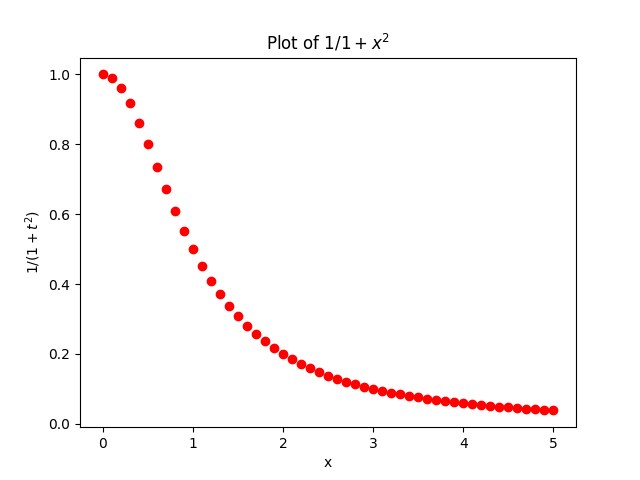
\includegraphics[width=0.5\textwidth, right]{Fig1.png}
\caption{Plot of f(x)=$\frac{1}{1+x^2}$}
\end{figure}

\section{Integrating the function and plotting error}
This question has three subparts in it:\\
1:Integrating the function from x=0 to x=5\\
2:Plotting the integral along with $\arctan(x)$\\
3:Plotting the error in the integral on a semilog axis.\\


\subsection{Part 1:}
For integrating the function we use \\
{\fontfamily{qcr}\selectfont
from scipy.integrate import quad}.The {\fontfamily{qcr}\selectfont quad} function takes in two arrays:\\
1:The function\\
2:The lower limit\\
3: The upper limit\\
The quad function integrates the values and returns the integral and the error in calculation.
Here we take lower limit=0 and upper limit=5.


\subsection{Part 2:}
The integrated function or the integral is plotted on red dots and the original function $\arctan(x)$ is plotted in a solid black line.
\begin{figure}[h!]
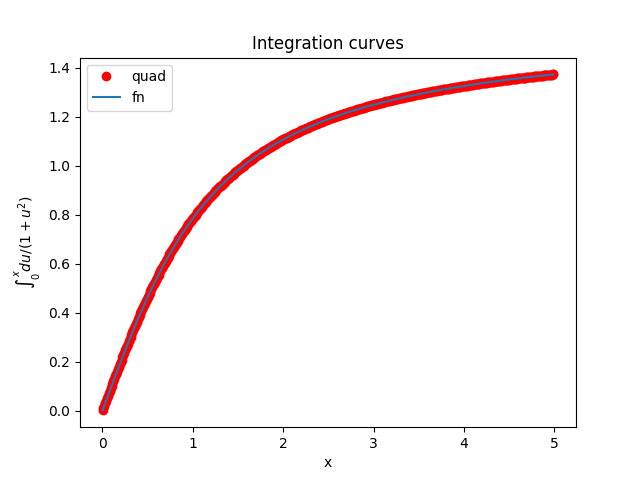
\includegraphics[width=0.5\textwidth, right]{Fig2.png}
 \caption{Plot of integrated function and $\arctan(x)$}
\end{figure}

\begin{figure}[h!]
  \includegraphics[width=0.5\textwidth, right]{Fig_table.png}
  \caption{Table of integrated function and $\arctan(x)$ for same x}
\end{figure}



\subsection{Part 3:}
The plot of the error in the integral is plotted on a semilog axis.It can be done by taking the absolute value of the difference between the calculated integral and the original function $\arctan(x)$. This can be dome by the following snippet of code:\\
\begin{verbatim}
import numpy as np
import matplotlib.pyplot as plt
error=np.abs(integrated-np.arctan(x_quad))
plt.semilogy(x_quad,error,'ro')
\end{verbatim}
\begin{figure}[h!]
  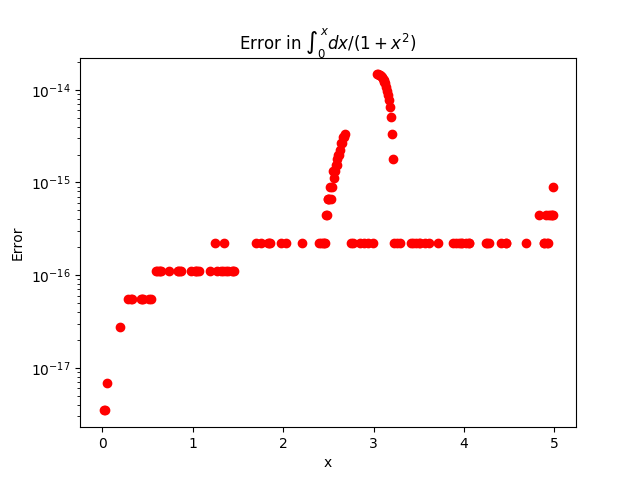
\includegraphics[width=0.4\textwidth, right]{Fig3.png}
  \caption{Plot or Error in the integration}
\end{figure}

\section{Integrating the function using Trapezoidal Method}
Trapezoidal Method is used for approximating a definite integral  I = $\int_{a}^{b} f(x)dx$ using linear approximations of the function f.
The trapezoids are drawn as shown below.\\
\begin{figure}[h!]
  \includegraphics[width=0.4\textwidth, right]{trapezoidal.png}
\end{figure}\\
The procedure for this method is as follows:\\
1: Partition [a,b] into the set $(X_0,X_1,X_2,......X_n) $so that there are n sub-intervals of equal width.\\
2: The integral $\int_{a}^{b} f(x)dx$ is estimated by adding the areas of all the trapezoids as illustrated above.The width of $\Delta{x}$ of each sub-interval given by $\Delta{x}$=$\frac{b-a}{n}$.\\
$\int_{a}^{b} f(x)dx$ = $\frac{\Delta{x}}{n} [ f(x_0)+2f(x_1)+2f(x_2)+...+2f(x_n-1)+f(x_n) ]$\\

The integration can be done by two methods:\\
1: Using a for loop\\
This is done by summing up the array of $f(x_i)$ for each i and storing in another array.After this $\frac{1}{2}(f(x_0)+f(x_n))$ is subtracted from that array.Then it is divided by $h$.
\\2: Vectorizing using {\fontfamily{qcr}\selectfont np.cumsum}
\\This is done by applying the {\fontfamily{qcr}\selectfont np.cumsum} function to the array containing $f(x_i)$ which would result in an array containing the summation part of the formula.
\\ The integrated function is then plotted.
\begin{figure}[h!]
  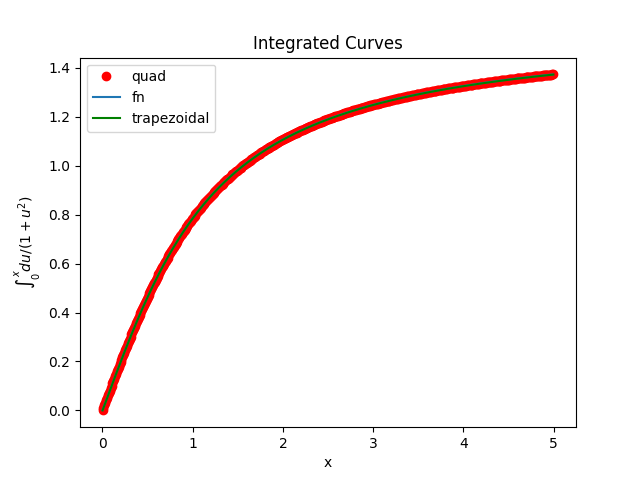
\includegraphics[width=0.4\textwidth, right]{Fig4.png}
  \caption{Plot of integrated function with  {\fontfamily{qcr}\selectfont quad},trapezoidal method and $\arctan(x)$}
\end{figure}

\section{Error Estimation in Trapezoidal Method}
\subsection{Estimated Error}
According to [1] and [2] the estimated error in trapezoidal method of integration for a continuous function $f(x)$ in the interval $a \leq x \leq b$ is:\\
$ E_h^T(f)=-\frac{h^2(b-a)}{12}f"(c_h)$ for some $c_h$ in the closed interval [a,b].
\\For our problem we have $f"(x) $ maximum at x=1 and it's value is $\frac{1}{2}$.
Thus by plugging in the values we get $|E_h^T(f)|=h^2\frac{5}{24}$

\subsection{Exact Error}
First of all an array containing the values of $h$ is made by halving it ten times.Then for each value of $h$ the integration value is calculated using the trapezoidal method.Then it is subtracted from $\arctan(x)$.Then the maximum absolute value of the error array is stored in 
{\fontfamily{qcr}\selectfont max\_error\_arr}.
\begin{figure}[h!]
  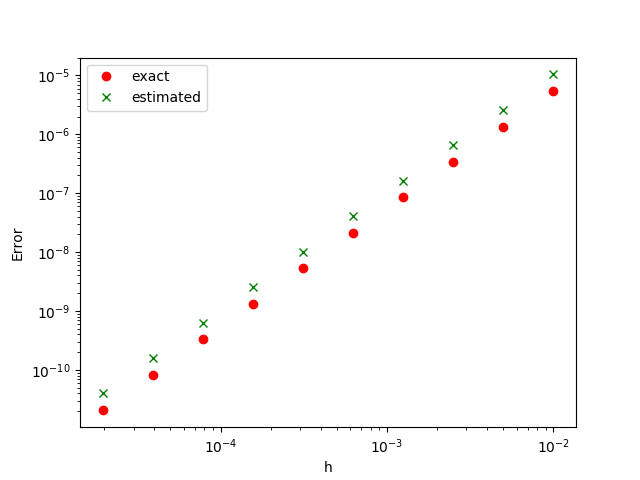
\includegraphics[width=0.4\textwidth, right]{Fig5.png}
  \caption{Estimated and Exact Errors}
\end{figure}

\section{References}
[1]:\url{http://homepage.divms.uiowa.edu/~atkinson/ftp/ENA_Materials/Overheads/sec_5-2.pdf}
\newline[2]:\url{http://math.cmu.edu/~mittal/Recitation_notes.pdf}
\end{document}